% Exact model a=3,b=2,u=9/4,v=1; component arrows are directed.
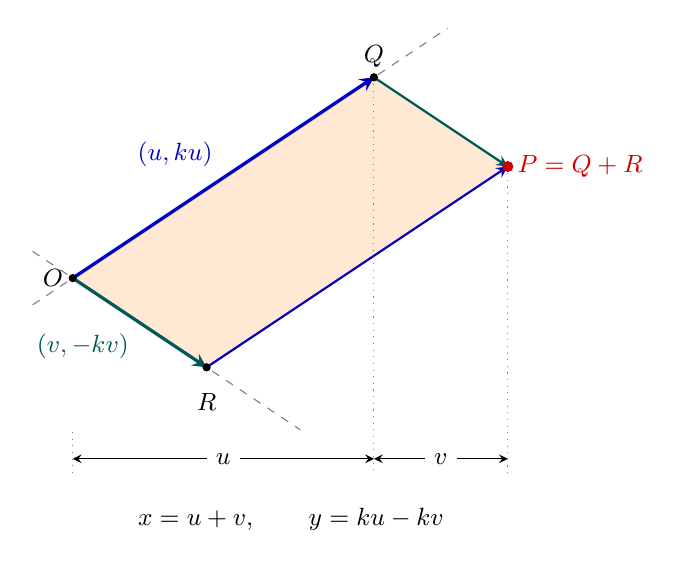
\begin{tikzpicture}[x=1.7cm,y=1.7cm,>=stealth,font=\small]
\coordinate (O) at (0,0); \coordinate (Q) at (2.25,1.5);
\coordinate (R) at (1,-2/3); \coordinate (P) at (3.25,5/6);
\fill[orange!17] (O)--(Q)--(P)--(R)--cycle;
\draw[gray,dashed] (-.3,-.2)--(2.8,28/15);
\draw[gray,dashed] (-.3,.2)--(1.7,-17/15);
\draw[->,blue!75!black,very thick] (O)--(Q) node[midway,above left] {$(u,ku)$};
\draw[->,teal!70!black,very thick] (O)--(R) node[midway,below left] {$(v,-kv)$};
\draw[->,teal!70!black,thick] (Q)--(P);
\draw[->,blue!75!black,thick] (R)--(P);
\draw[gray,dotted] (0,-1.15)--(0,-1.45) (Q)--(2.25,-1.45) (P)--(3.25,-1.45);
\draw[<->] (0,-1.35)--(2.25,-1.35) node[midway,fill=white] {$u$};
\draw[<->] (2.25,-1.35)--(3.25,-1.35) node[midway,fill=white] {$v$};
\node at (1.63,-1.8) {$x=u+v,\qquad y=ku-kv$};
\fill (O) circle(1.5pt) node[left] {$O$};
\fill (Q) circle(1.5pt) node[above] {$Q$};
\fill (R) circle(1.5pt) node[below=6pt] {$R$};
\fill[red!80!black] (P) circle(2pt) node[right] {$P=Q+R$};
\end{tikzpicture}
